\documentclass[12pt,a4paper]{article}
\usepackage{ctex}
%\usepackage{geometry}
%\bibliographystyle{plain}
\usepackage[super]{gbt7714}
%\geometry{a4paper}
\usepackage[margin=2.3cm]{geometry}
\usepackage{graphicx}
\usepackage{float}%强制左对齐1
\usepackage{longtable}
\usepackage{listings} 
\usepackage{graphicx}
\graphicspath{{figures/}}
%\usepackage{biblatex}
\usepackage{amsmath}
\usepackage{amsfonts}
\usepackage{booktabs}
\usepackage{xcolor}
\usepackage{soul}
\title{\heiti 实验一 \quad 遥感软件与遥感数据认识}
\author{}

\date{ }


\newcommand{\upcite}[1]{\textsuperscript{\textsuperscript{\cite{#1}}}} 

\def\degree{${}^{\circ}$}
\definecolor{Seashell}{RGB}{255, 245, 238} %背景色浅一点的
\definecolor{Firebrick4}{RGB}{255, 0, 0}%文字颜色红一点的
\newcommand{\code}[1]{
	\begingroup
	\sethlcolor{Seashell}%背景色
	\textcolor{Firebrick4}{\hl{#1}}%textcolor里面对应文字颜色
	\endgroup
}


\begin{document}
	
	\maketitle	
	

\leftline{\textbf{实验时间}:2021年11月19日}	
\leftline{\textbf{实验环境}:电脑:Windows 10(64 bit); \quad 软件: ENVI 5.3 \quad SP1(64bit)}	
	
	\section{实验要求}
		\begin{enumerate}
		
		\item 进行遥感实验的初步准备,安装ENVI软件,证明成功启动ENVI,然后文档编辑描逑安装过程,撰写入实验报告。
		
		
		\item 成功从‘地理空间云’中下载自己家乡的Landsat8数据,说明数据查询和下载的方法,撰写入实验报告。
			
		
		
		
		
	\end{enumerate}
	
	\section{实验步骤}
	
	
	\subsection{安装ENVI 5.3(64bit)}
	
		(1)打开ENVI安装文件,点击\code{IDL\_ENVI53SP1win64.exe} 开始安装
		
		\begin{figure}[H]
			\centering
			\begin{minipage}[t]{0.48\textwidth}
				\centering
				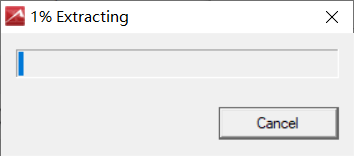
\includegraphics[width=5.0cm]{ins}	
			\end{minipage}
			\begin{minipage}[t]{0.48\textwidth}
				\centering 
				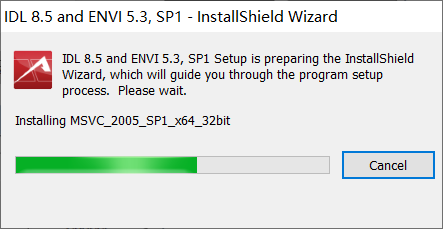
\includegraphics[width=5.0cm]{ins2}
			\end{minipage}
		\end{figure}
		
		(2)进行相关的设置,设置安装路径
		
		\begin{figure}[H]
			\centering
			\begin{minipage}[t]{0.48\textwidth}
				\centering
				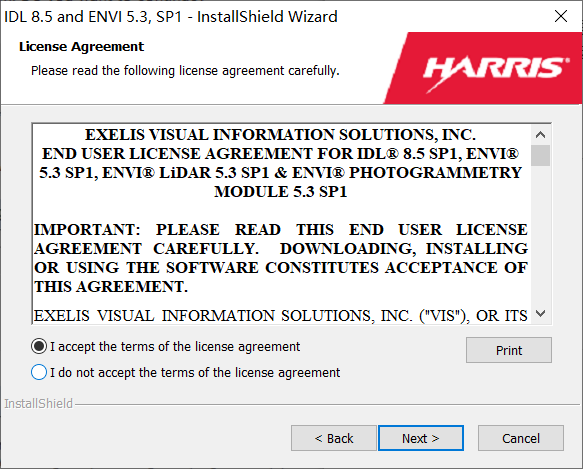
\includegraphics[height=4.0cm]{ins3}	
			\end{minipage}
			\begin{minipage}[t]{0.48\textwidth}
				\centering 
				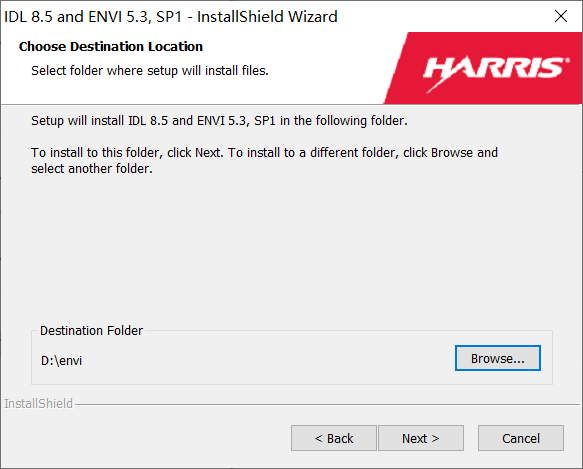
\includegraphics[height=4.0cm]{ins4}
			\end{minipage}
		\end{figure}
	
		(3)进行软件的授权,最终软件安装完成
	
	\begin{figure}[H]
		\centering
		\begin{minipage}[t]{0.48\textwidth}
			\centering
			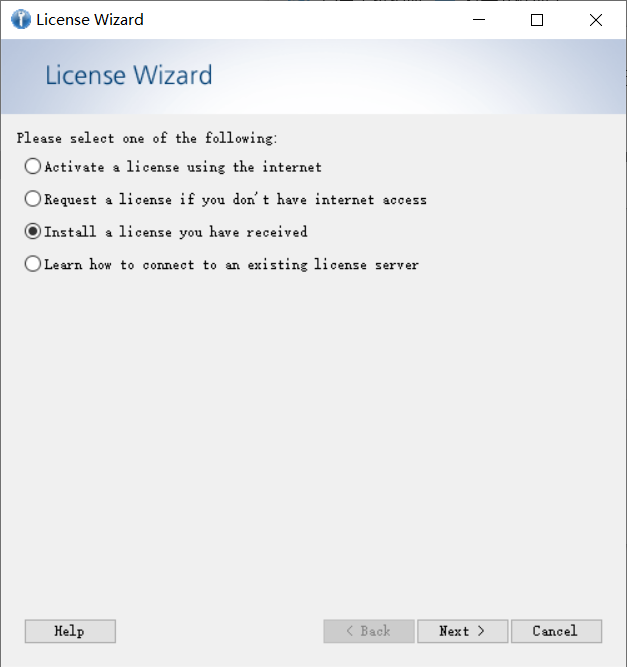
\includegraphics[height=4.0cm]{ins5}	
		\end{minipage}
		\begin{minipage}[t]{0.48\textwidth}
			\centering 
			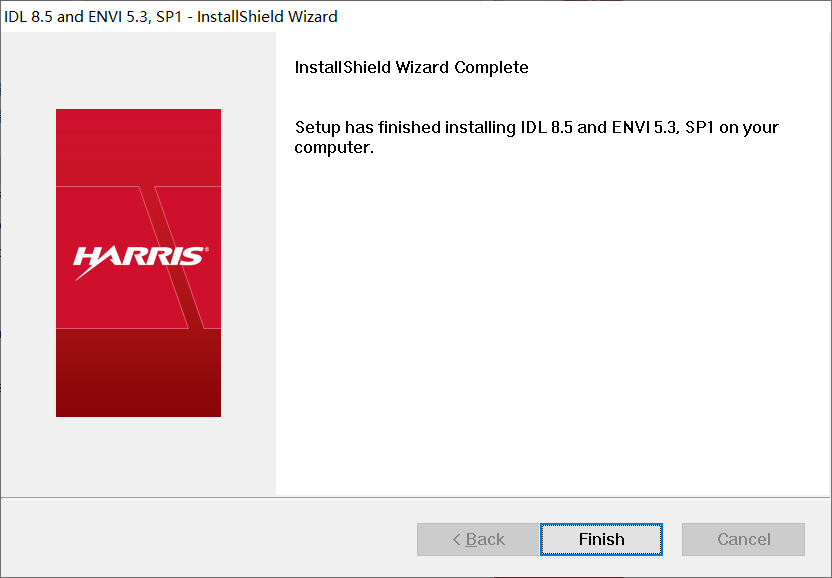
\includegraphics[height=4.0cm]{ins6}
		\end{minipage}
	\end{figure}
	
	(4)打开软件的初始界面
	\begin{figure}[H]
		\centering
		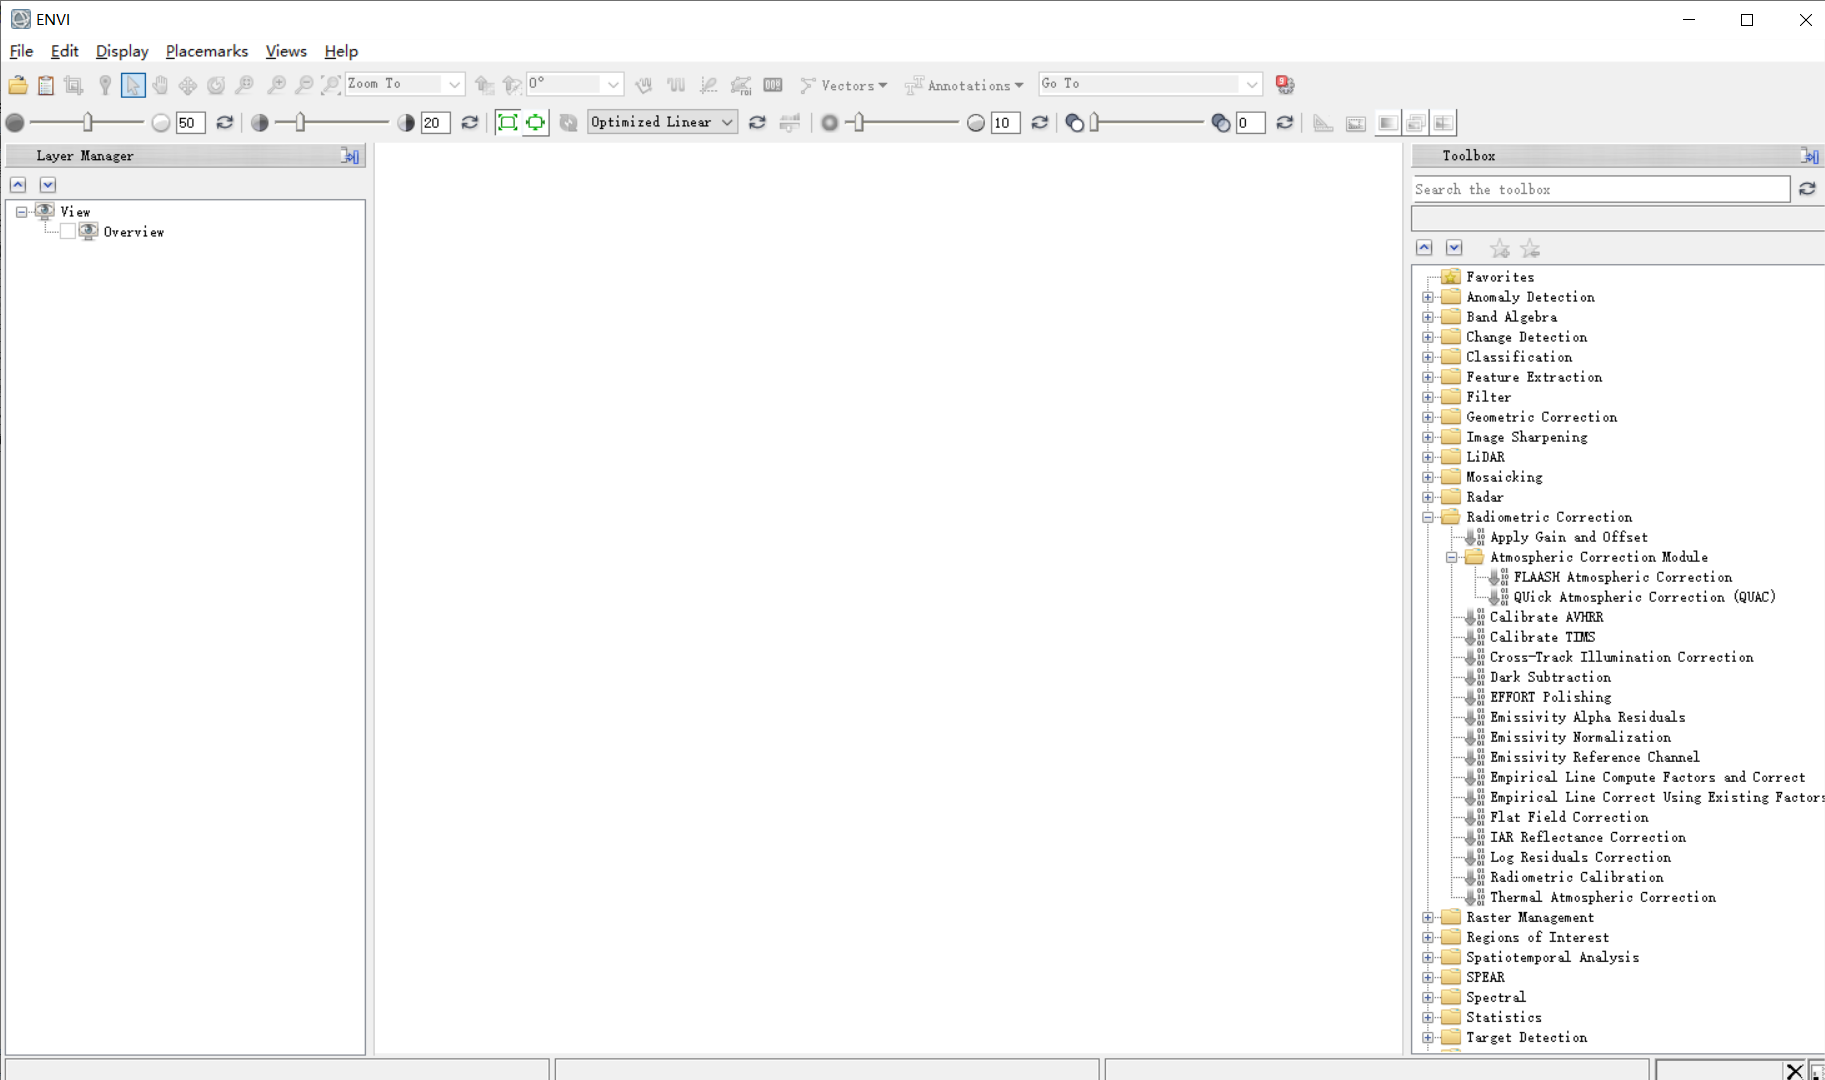
\includegraphics[width=.7\textwidth]{all}
		\caption{ENVI 5.3 (64bit)界面}
		\label{fig:we}
	\end{figure}
	
	\subsection{在地理空间数据云下载\textit{安徽省宣城市}遥感影像}
	
	
	
	(1)打开\textbf{地理空间数据云门户网站}(\underline{http://www.gscloud.cn}),选择\textbf{高级检索}。
	\begin{figure}[H]
		\centering
		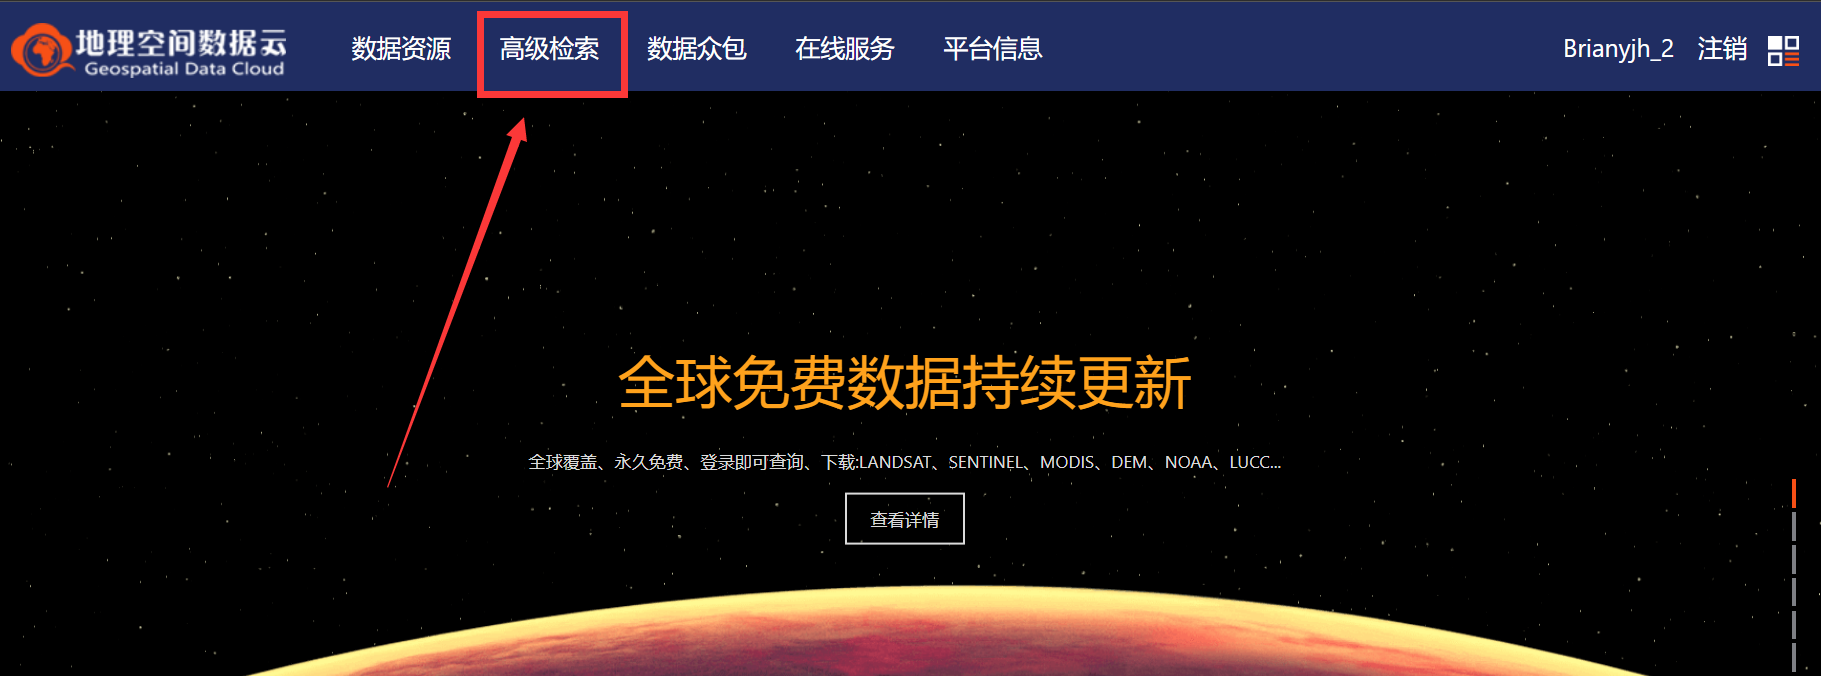
\includegraphics[width=.7\textwidth]{web}
		\caption{地理空间数据云门户网站页面}
		\label{fig:web}
	\end{figure}
	
	(2)在高级检索中,\textbf{数据集}选择\textit{Landsat 8 OLI\_TIRS 卫星数字产品},\textbf{空间位置}选择\textit{矩形},在地图划定区域,为了方便后续实验处理,限制\textbf{云量}在\textit{0.5}以下。
	
	
	\begin{figure}[H]
		\centering
		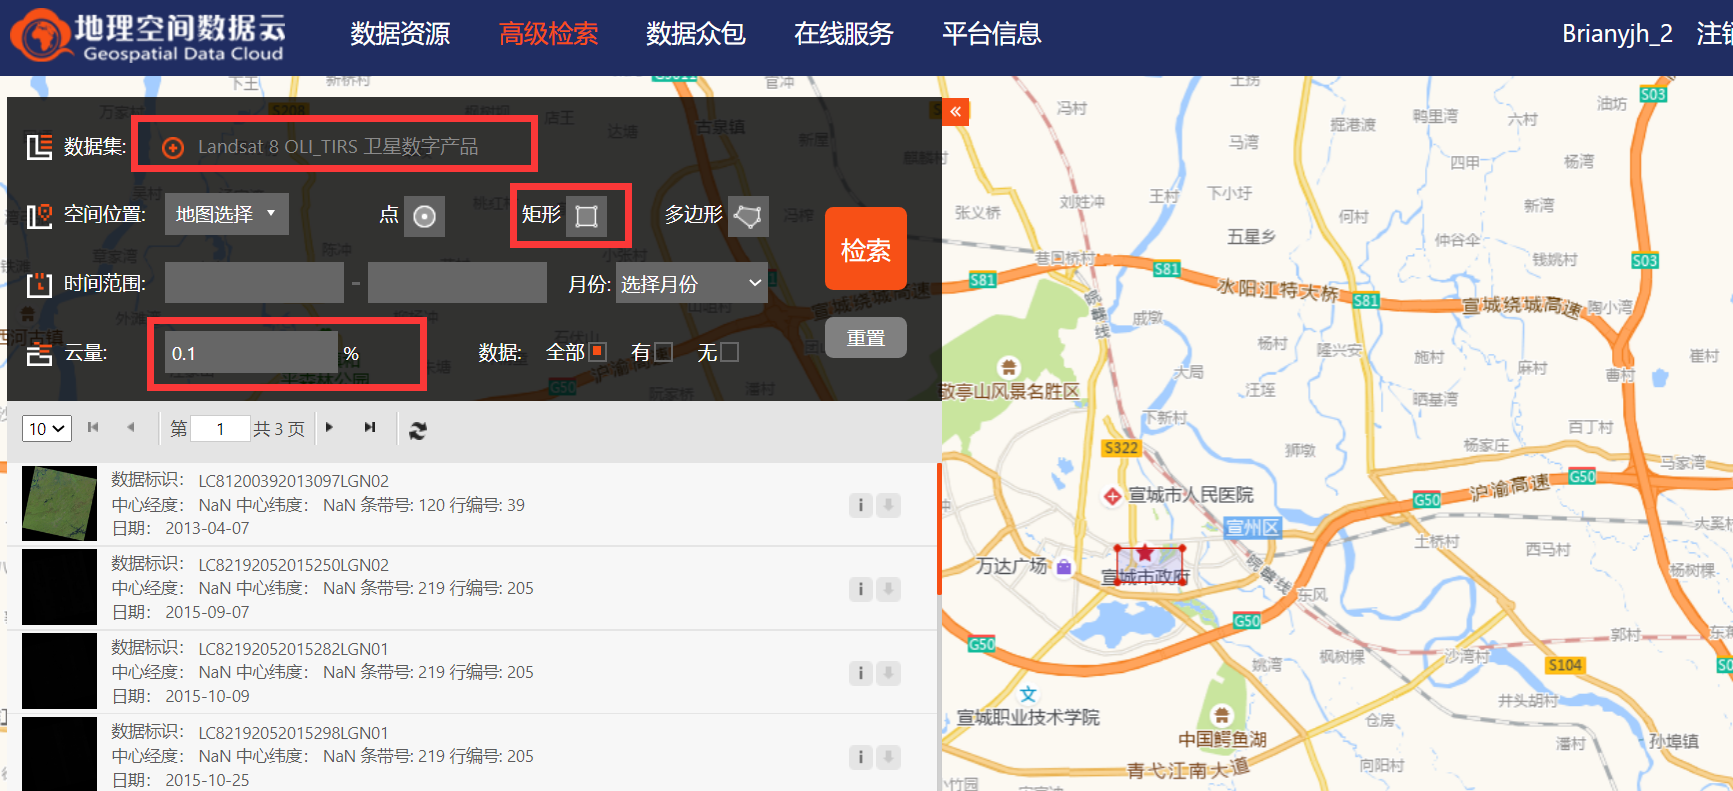
\includegraphics[width=.7\textwidth]{web_select}
		\caption{高级检索页面}
		\label{fig:web2}
	\end{figure}
	
	(3)在检索结果中,可以清晰看到符合条件的数据集的\textit{数据标识}、\textit{中心经度}、\textit{条带号}、\textit{行编号}以及\textit{日期},点击\textit{倒感叹号按钮}可以查看数据集的详细参数,点击\textit{下载按钮}可以下载数据(如果按钮是灰色则无法下载),在右侧可以看到数据的\textit{大致范围}。
	
	\begin{figure}[H]
		\centering
		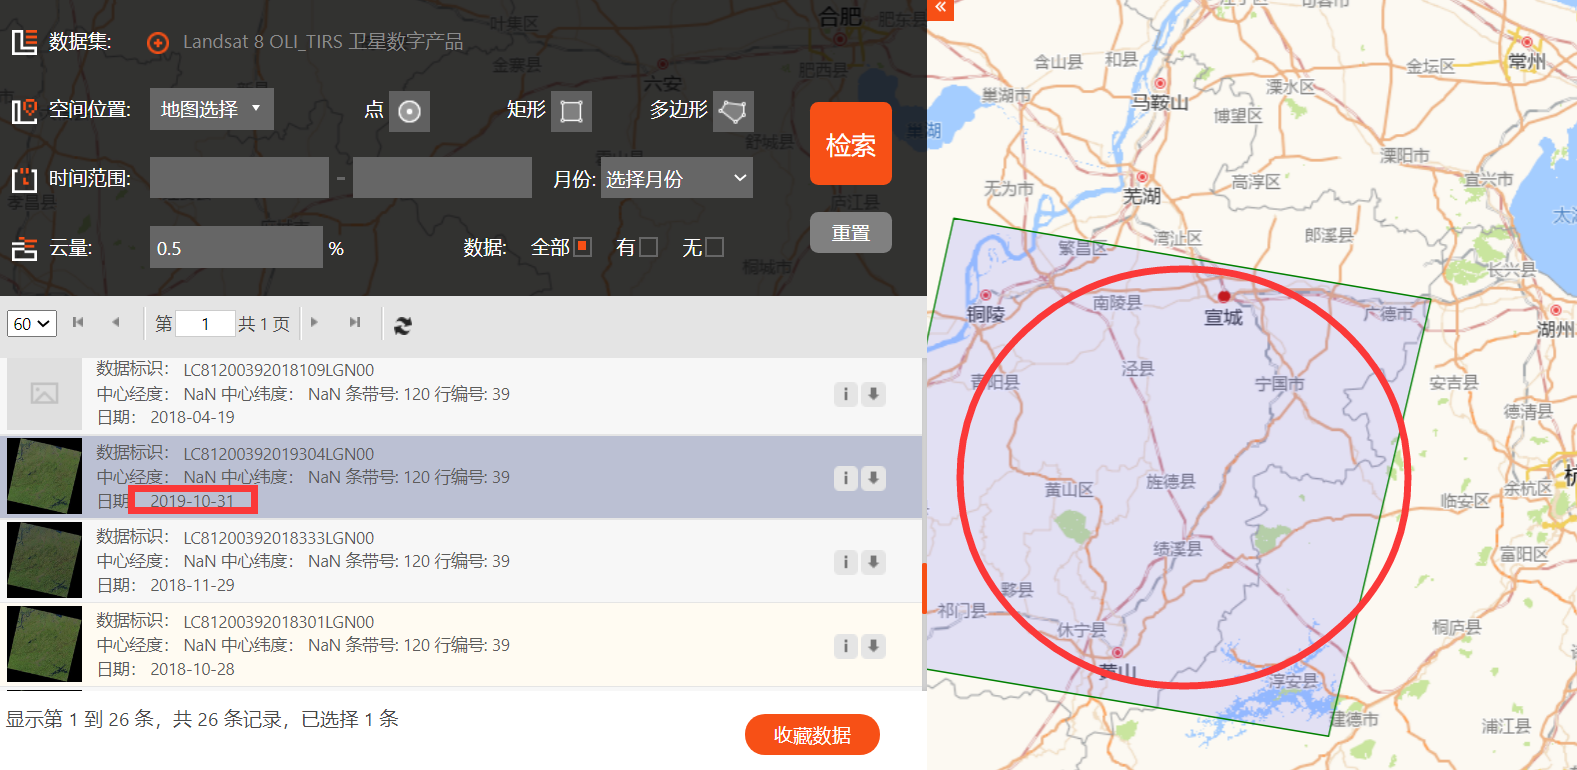
\includegraphics[width=.7\textwidth]{web_select2}
		\caption{检索结果}
		\label{fig:web3}
	\end{figure}
	\begin{figure}[H]
		\centering
		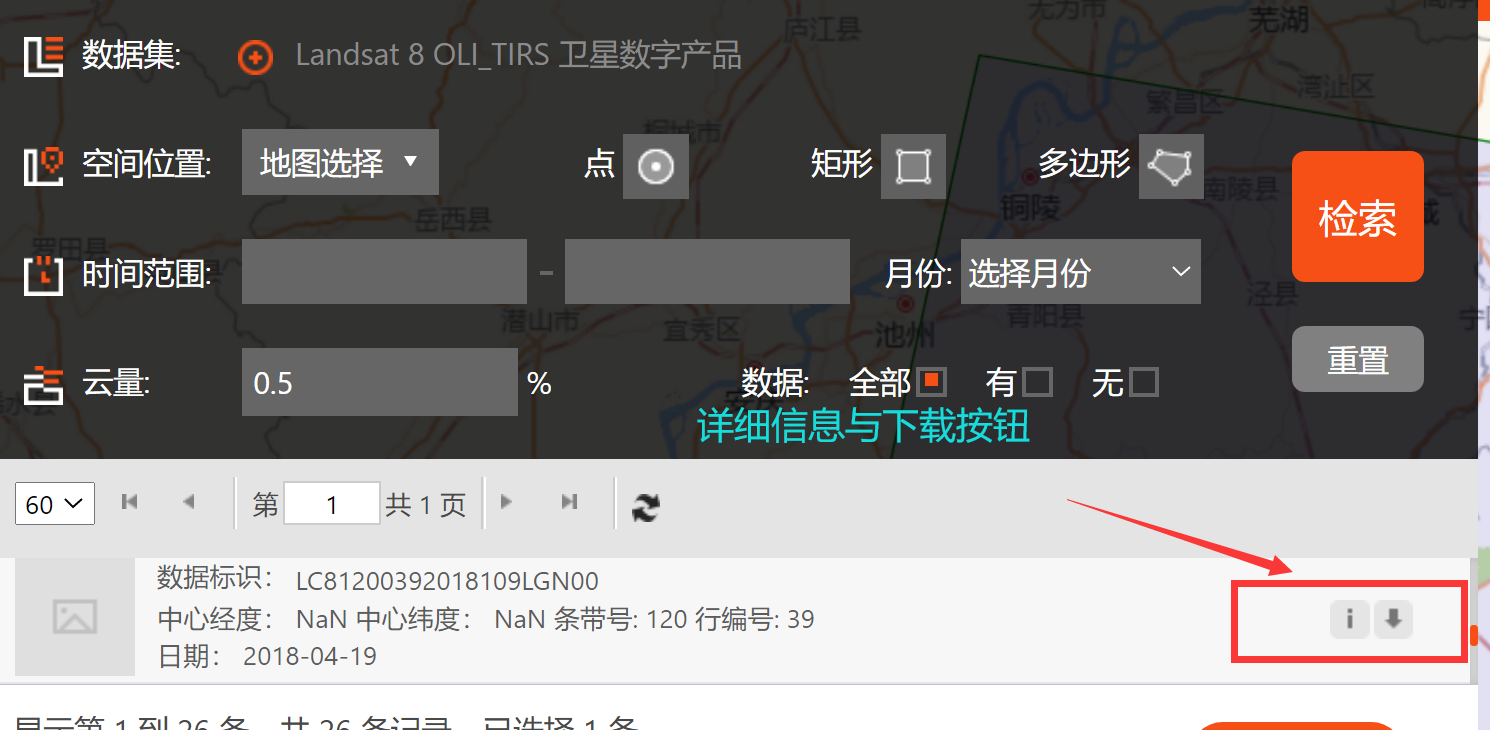
\includegraphics[width=.7\textwidth]{3}
		\caption{详细信息与下载按钮}
		\label{fig:web4}
	\end{figure}
	
	
	(4)选定相对近期的时间的数据(\textit{2019-10-31}),点击\textit{下载按钮}开始下载
	
	\begin{figure}[H]
		\centering
		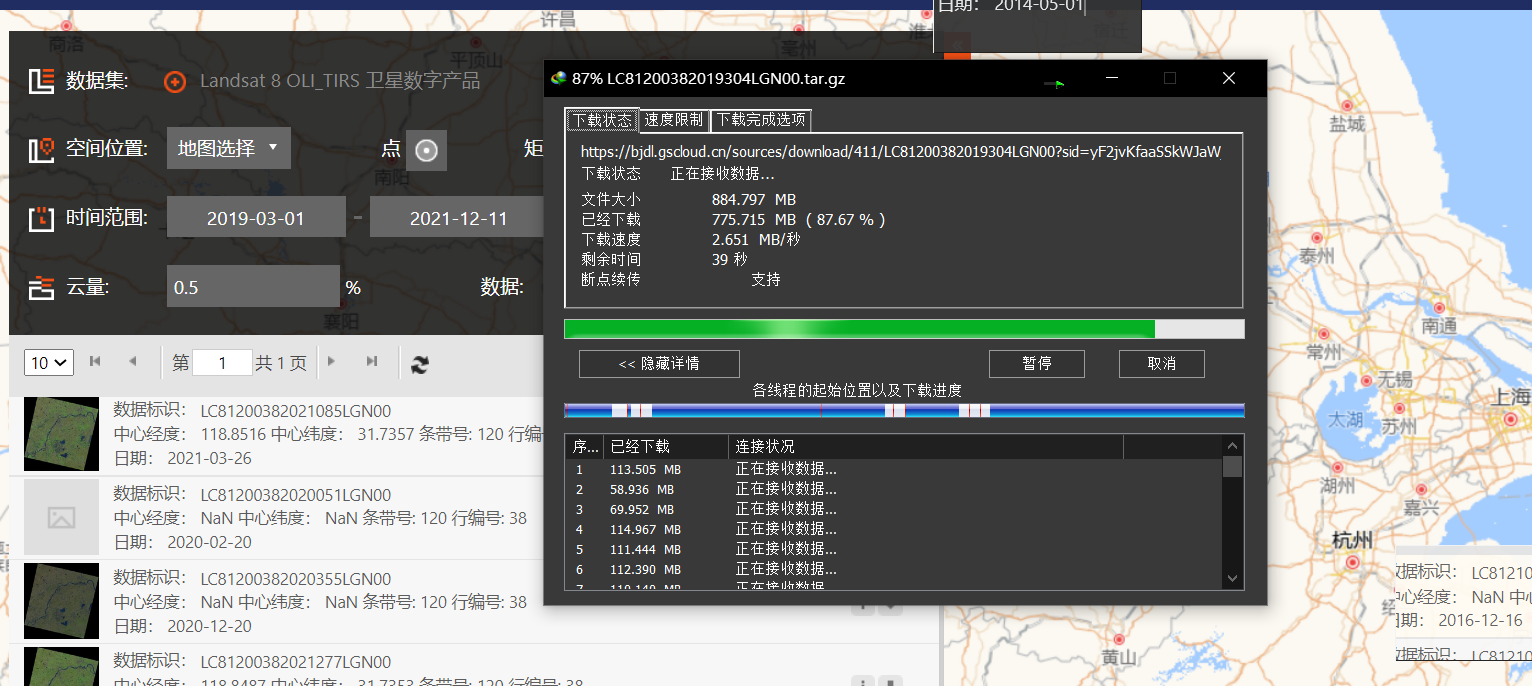
\includegraphics[width=.7\textwidth]{2}
		\caption{下载过程}
		\label{fig:web4}
	\end{figure}
	

	
	
	
	
	
	\section{实验结果}
	
	
	将下载的数据进行解压后得到我们需要的宣城市的遥感影像
	
		\begin{figure}[H]
		\centering
		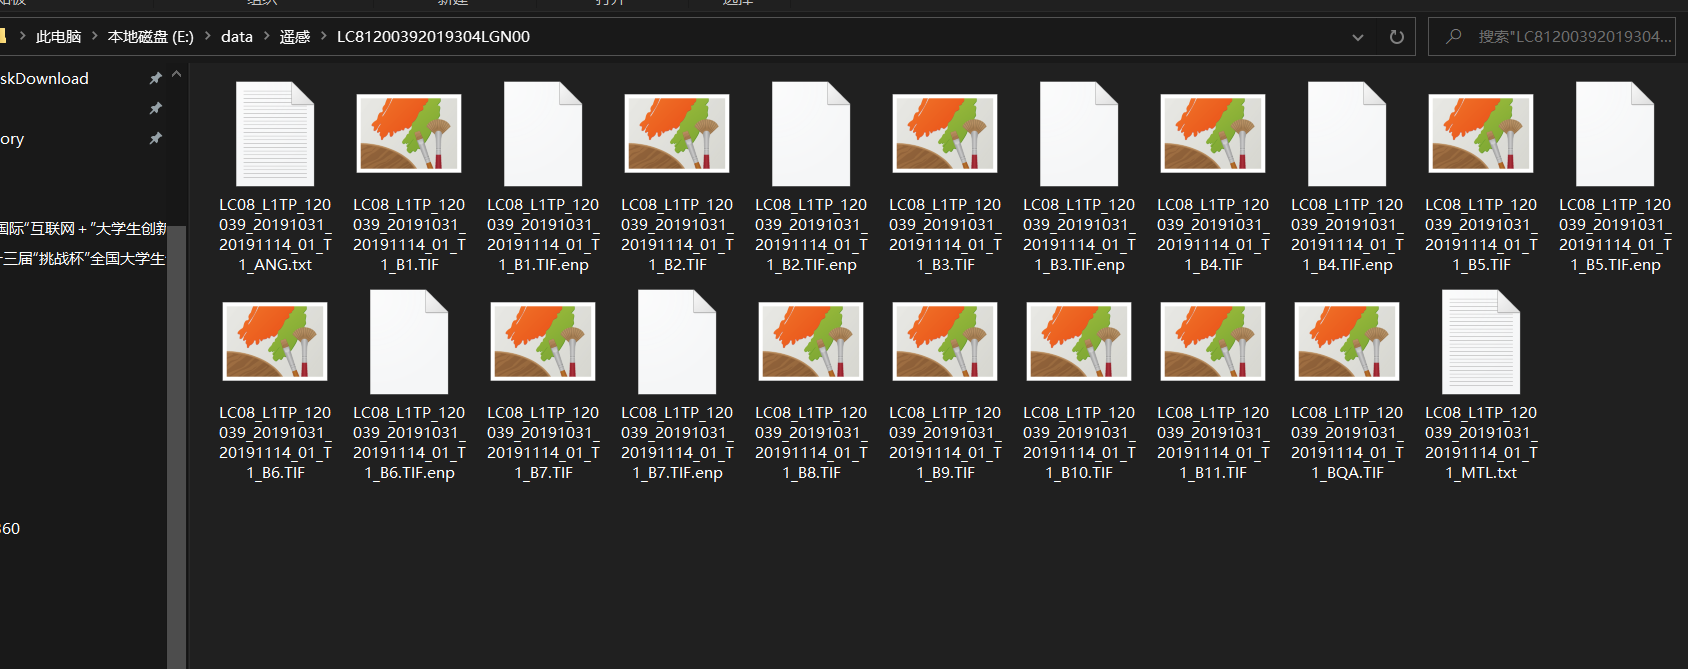
\includegraphics[width=.7\textwidth]{res1}
		\caption{遥感数据文件}
		\label{fig:web4}
	\end{figure}
	
	
	

	

		
	
		
	\end{document}